\section{Program} 
The program we have implemented had 2 important parts: 
The first one is to recognize the face of a person, and to do that we use python with opencv libraries.

The second part of our project regards the model we use to estimate if a person is wearing a mask. We used the RES-Net 50 convolution neural network to create and train our model. Since the model created is very heavy we had to fine-tune it in order to implement it in our program.

The RES-Net 50 model that we created works really well with the dataset that we have used. We split data in 60 - 20 - 20 train-validation-test and the accuracy of the test set is 0.98.
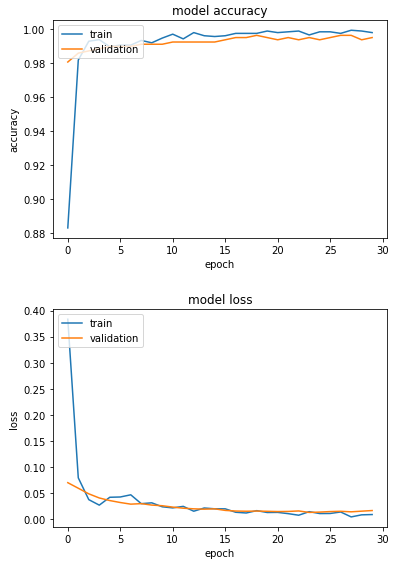
\includegraphics{LossAndAccuracy}

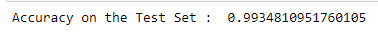
\includegraphics{testAccuracy}